\section{Mess-/Steuerkette} \label{cpt:MessSteuerkette}


\begin{figure}[H]
	\begin{center}
		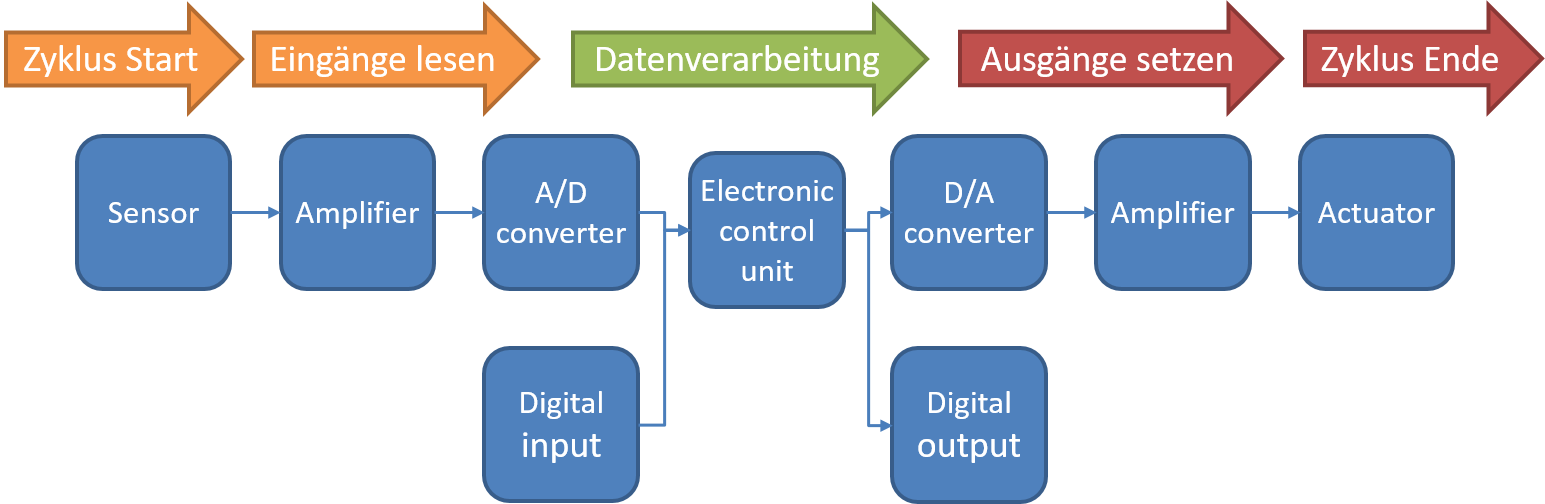
\includegraphics[width=0.7\textwidth]{images/Messsteuerkette.png}
		\caption{Blockschaltbild des FB für die Betriebszustandsampel.}
		\label{fig:Messsteuerkette}
	\end{center}	
\end{figure}


\subsection{Sensoren \& Eingangssignale}

\subsection{Aktoren \& Ausgangssignale}

\subsection{E/A - Klemmen}

\subsection{Datenaufzeichnung - Scope Baustein}

\subsection{Reglerimplementierung}

\subsection{Optionale Aufgaben}

\subsubsection{Füllmengenkalibrierung - 10 Punkte}

\subsubsection{PI-Temperaturregler - 10 Punkte}


\newpage
